La siguiente pirámide cuadrangular tiene base con lados de 10 unidades de longitud.
La altura inclinada de la pirámide es 8 unidades, como se muestra en la figura \ref{fig:pitagoras3D_piram_02}:\\
\begin{figure}[H]
    \begin{center}
        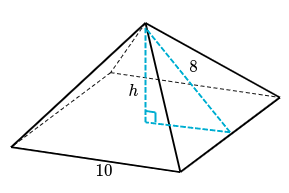
\includegraphics[width=0.3\textwidth]{../images/pitagoras3D_piram_02.png}
    \end{center}
    \caption{}
    \label{fig:pitagoras3D_piram_02}
\end{figure}
\textbf{¿Cuál es la altura vertical $h$?}\\
\textit{Redondea tu respuesta a la décima más cercana.}